\newcommand{\ablA}{2747}
\newcommand{\ablB}{1869}
\newcommand{\ablC}{1589}
\newcommand{\ablD}{497}
\newcommand{\ablDicomC}{15325}
\newcommand{\ablDicomD}{2150}
\newcommand{\ablRatio}{5.5}
\newcommand{\ablRatioNb}{3.2}
\newcommand{\auxBASE}{111.7k}
\newcommand{\auxQeight}{365}
\newcommand{\auxQfour}{561}
\newcommand{\auxQtwo}{1659}
\newcommand{\auxRatio}{199}
\newcommand{\auxReight}{429}
\newcommand{\auxRfour}{610}
\newcommand{\auxRtwo}{928}
\newcommand{\berinnQeight}{0.44}
\newcommand{\berinnQfour}{3.04}
\newcommand{\berinnQtwo}{7.34}
\newcommand{\berinnReight}{0.23}
\newcommand{\berinnRfour}{2.05}
\newcommand{\berinnRtwo}{4.19}
\newcommand{\capPEE}{9.6k}
\newcommand{\exactBASE}{0}
\newcommand{\exactPEE}{393}
\newcommand{\exactQ}{385}
\newcommand{\exactR}{371}
\newcommand{\failBASE}{132}
\newcommand{\failPEE}{3}
\newcommand{\failQ}{11}
\newcommand{\failR}{25}
\newcommand{\nImgs}{132}
\newcommand{\okBASE}{0}
\newcommand{\okPEE}{393}
\newcommand{\okQ}{385}
\newcommand{\okR}{371}
\newcommand{\pinnBASE}{46.07}
\newcommand{\pinnQeight}{50.16}
\newcommand{\pinnQfour}{49.40}
\newcommand{\pinnQtwo}{46.64}
\newcommand{\pinnReight}{49.26}
\newcommand{\pinnRfour}{47.92}
\newcommand{\pinnRtwo}{43.49}
\newcommand{\psnrPEEeight}{71.64}
\newcommand{\psnrPEEfour}{65.32}
\newcommand{\psnrPEEtwo}{57.84}
\newcommand{\psnrQeight}{49.92}
\newcommand{\psnrQfour}{49.05}
\newcommand{\psnrQtwo}{45.73}
\newcommand{\psnrReight}{49.03}
\newcommand{\psnrRfour}{47.57}
\newcommand{\psnrRtwo}{42.94}
\newcommand{\resBASE}{36}
\newcommand{\robgaussonePEE}{50.17}
\newcommand{\robgaussoneQ}{2.07}
\newcommand{\robgaussoneR}{1.26}
\newcommand{\robgaussthreePEE}{50.05}
\newcommand{\robgaussthreeQ}{6.30}
\newcommand{\robgaussthreeR}{3.62}
\newcommand{\robgausstwoPEE}{49.87}
\newcommand{\robgausstwoQ}{3.22}
\newcommand{\robgausstwoR}{1.76}
\newcommand{\robjpegeightyPEE}{50.04}
\newcommand{\robjpegeightyQ}{47.02}
\newcommand{\robjpegeightyR}{46.10}
\newcommand{\robjpegnfPEE}{50.15}
\newcommand{\robjpegnfQ}{12.14}
\newcommand{\robjpegnfR}{5.07}
\newcommand{\robjpegninetyPEE}{50.47}
\newcommand{\robjpegninetyQ}{38.74}
\newcommand{\robjpegninetyR}{36.07}
\newcommand{\robnonezeroPEE}{0.00}
\newcommand{\robnonezeroQ}{1.78}
\newcommand{\robnonezeroR}{1.16}
\newcommand{\robspsphalfPEE}{48.29}
\newcommand{\robspsphalfQ}{3.35}
\newcommand{\robspsphalfR}{2.17}
\newcommand{\robspsponePEE}{48.99}
\newcommand{\robspsponeQ}{6.10}
\newcommand{\robspsponeR}{4.03}
\newcommand{\runsBASE}{132}
\newcommand{\runsPEE}{396}
\newcommand{\runsQ}{396}
\newcommand{\runsR}{396}
\newcommand{\ssimPEEeight}{0.9999}
\newcommand{\ssimPEEfour}{0.9998}
\newcommand{\ssimPEEtwo}{0.9991}
\newcommand{\ssimQeight}{0.9960}
\newcommand{\ssimQfour}{0.9949}
\newcommand{\ssimQtwo}{0.9896}
\newcommand{\ssimReight}{0.9955}
\newcommand{\ssimRfour}{0.9940}
\newcommand{\ssimRtwo}{0.9821}
\newcommand{\tembPEEeight}{0.02}
\newcommand{\tembPEEfour}{0.02}
\newcommand{\tembPEEtwo}{0.02}
\newcommand{\tembQeight}{0.49}
\newcommand{\tembQfour}{0.51}
\newcommand{\tembQtwo}{0.59}
\newcommand{\tembReight}{0.49}
\newcommand{\tembRfour}{0.51}
\newcommand{\tembRtwo}{0.56}
\newcommand{\textPEEeight}{0.02}
\newcommand{\textPEEfour}{0.02}
\newcommand{\textPEEtwo}{0.02}
\newcommand{\textQeight}{0.48}
\newcommand{\textQfour}{0.51}
\newcommand{\textQtwo}{0.59}
\newcommand{\textReight}{0.49}
\newcommand{\textRfour}{0.51}
\newcommand{\textRtwo}{0.56}

\section{Experimental Results and Analysis}
\subsection{Setup}
\textbf{Data.} Training uses the 100 Urban100 images~\cite{huang2015urban} converted to grey (92 for training, 8 for
validation) with random $64\times64$ crops and flips. Testing uses three sets that never appear in training: BSD100
\cite{martin2001bsd} ($256\times256$ centre crops), the 24 Kodak images~\cite{kodak} (grey, $512\times512$ centre crop
resized to $256\times256$, as is common practice for BOSSbase~\cite{bas2011boss}) and 8 real DICOM slices (3 CT, 2 MR,
2 CR, 1 perfusion CT) from the public pydicom test collection~\cite{pydicomdata}, windowed to 8 bits and resized to
$256\times256$. This gives \nImgs{} test images. BOSSbase 1.01 was not reachable from our network; the scripts accept
any folder of images.

\textbf{Training.} Both IC-INN models are trained for 12{,}000 iterations, batch 12, Adam~\cite{kingma2015adam} with a
cosine schedule from $10^{-3}$, on a 2-core CPU (about 15 minutes each). Fig.~\ref{fig:train} shows the curriculum: the
stego PSNR first drops while the decoder learns, then rises as the image loss is switched on.

\textbf{Compared methods.} (i) Rhombus PEE~\cite{sachnev2009} embedding the message directly, using our implementation
(the same one used for the side information). (ii) A float-INN baseline with residual compensation: a HiNet-style
\cite{jing2021hinet} affine-coupling network in the Haar domain (128.7k parameters), trained with rounding in the loop and
a cover-recovery loss; its residual $X-\lfloor 255\hat X\rceil$ and wrong bits are coded and hidden by PEE in the same way
as ours. (iii) IC-INN-Q and (iv) IC-INN-R, our quality- and robustness-oriented models.

\textbf{Metrics and payloads.} Payloads are 256, 1024 and 4096 bits ($s=8,4,2$), i.e.\ 0.0039, 0.0156 and 0.0625 bpp
of message on a $256\times256$ cover. We report PSNR and SSIM~\cite{wang2004ssim} of the final stego against the cover,
the side-information size, BER and NC of the extracted message, and whether the cover came back bit for bit. A run counts
as exact only if both \texttt{isequal(cover, recovered)} and \texttt{isequal(message, extracted)} hold in MATLAB.

\subsection{Reversibility and image quality}
Table~\ref{tab:main} lists the lossless results. Every run that finished embedding was exactly reversible:
\exactQ{} of \runsQ{} runs for IC-INN-Q and \exactR{} of \runsR{} for IC-INN-R, with BER $=0$ and NC $=1$ in all of them,
on natural and medical images alike. The remaining runs (\failQ{} and \failR{}) failed \emph{before} embedding because
the side information did not fit into the PEE capacity of the image; this happens only for busy textures or noisy dark
scans at the largest payload, and the sender detects it. Classical PEE fails on \failPEE{} runs for the same reason.

At 1024 bits IC-INN-Q reaches \psnrQfour{}~dB and SSIM \ssimQfour{}; at 4096 bits \psnrQtwo{}~dB and \ssimQtwo{}.
Before the side information is added the stego has \pinnQfour{} and \pinnQtwo{}~dB, so the compensation stage costs
less than 1~dB. The side information is smaller than the message it protects: on average \auxQfour{} bits for a
1024-bit message and \auxQtwo{} bits for a 4096-bit one. Fig.~\ref{fig:psnr} shows PSNR and side-information size against
payload, and Fig.~\ref{fig:visual} shows examples; the difference images are noise-like, with no visible structure.

Classical PEE gives much higher PSNR at these small payloads (\psnrPEEfour{}~dB at 1024 bits). This is expected and we do
not hide it: when the channel is guaranteed lossless, prediction-error expansion changes only a few hundred pixels by
one level, while a learned embedding spreads a decodable signal over the whole image. The point of the learned embedding
is what happens when the channel is \emph{not} lossless (Section~\ref{sec:robust}).

\begin{table*}[t]
\centering
\caption{Lossless results per test set and payload (mean over images). Aux = side-information bits embedded by PEE; Exact = images whose cover \emph{and} message were recovered bit for bit. Lossless BER was 0 and NC was 1 for every exact case.}
\label{tab:main}
\setlength{\tabcolsep}{3.2pt}
\begin{tabular}{lcc|ccc|cccc|cccc}
\toprule
& & & \multicolumn{3}{c|}{Rhombus PEE \cite{sachnev2009}} & \multicolumn{4}{c|}{IC-INN-Q (ours)} & \multicolumn{4}{c}{IC-INN-R (ours)}\\
Set & Bits & bpp & PSNR & SSIM & Exact & PSNR & SSIM & Aux & Exact & PSNR & SSIM & Aux & Exact\\
\midrule
BSD100 & 256 & 0.0039 & 71.30 & 0.9999 & 100/100 & 49.87 & 0.9971 & 310 & 99/100 & 48.96 & 0.9965 & 327 & 99/100\\
 & 1024 & 0.0156 & 64.91 & 0.9998 & 100/100 & 49.00 & 0.9960 & 459 & 99/100 & 47.52 & 0.9948 & 499 & 98/100\\
 & 4096 & 0.0625 & 57.24 & 0.9991 & 98/100 & 45.69 & 0.9904 & 1608 & 95/100 & 42.87 & 0.9827 & 980 & 89/100\\
\midrule
Kodak & 256 & 0.0039 & 71.98 & 0.9999 & 24/24 & 50.25 & 0.9966 & 334 & 24/24 & 49.33 & 0.9959 & 353 & 24/24\\
 & 1024 & 0.0156 & 65.88 & 0.9998 & 24/24 & 49.31 & 0.9954 & 438 & 24/24 & 47.79 & 0.9936 & 535 & 24/24\\
 & 4096 & 0.0625 & 58.70 & 0.9991 & 23/24 & 46.03 & 0.9895 & 1191 & 23/24 & 43.15 & 0.9797 & 731 & 22/24\\
\midrule
DICOM & 256 & 0.0039 & 74.77 & 1.0000 & 8/8 & 49.51 & 0.9799 & 1137 & 8/8 & 49.09 & 0.9820 & 1918 & 8/8\\
 & 1024 & 0.0156 & 68.78 & 0.9998 & 8/8 & 48.87 & 0.9802 & 2191 & 8/8 & 47.50 & 0.9817 & 2730 & 6/8\\
 & 4096 & 0.0625 & 62.63 & 0.9989 & 8/8 & 45.23 & 0.9738 & 4791 & 5/8 & 43.94 & 0.9789 & 640 & 1/8\\
\bottomrule
\end{tabular}
\end{table*}


\begin{figure}[t]
\centering
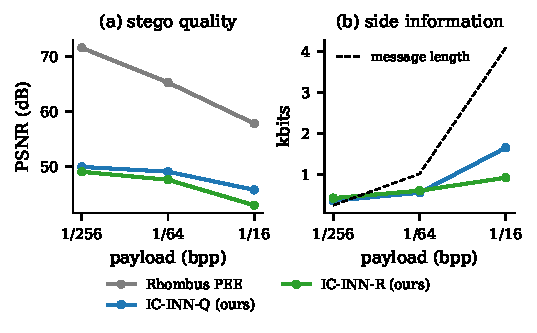
\includegraphics[width=\columnwidth]{figs/psnr_bpp.pdf}
\caption{(a) Mean stego PSNR over all test images versus payload. (b) Mean side-information size; the dashed line is
the message length.}
\label{fig:psnr}
\end{figure}

\begin{figure}[t]
\centering
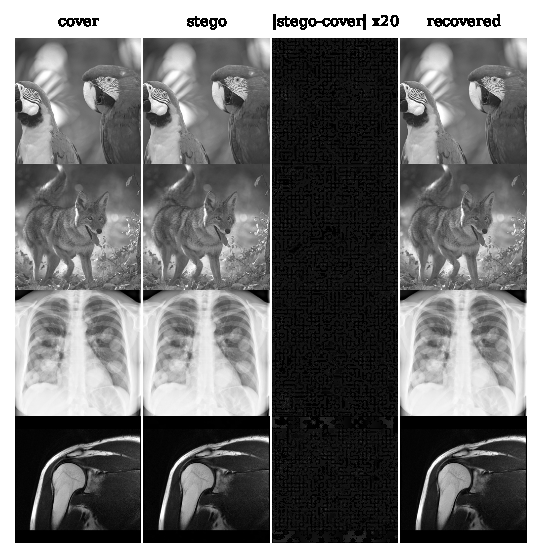
\includegraphics[width=0.92\columnwidth]{figs/visual.pdf}
\caption{IC-INN-Q at 1024 bits (Kodak 23, BSD100 \#10, chest CR, shoulder MR). The recovered images are identical to
the covers.}
\label{fig:visual}
\end{figure}

\subsection{Side-information coding (ablation)}
Table~\ref{tab:ablation} isolates the coder. Without entropy coding (A0) the side information averages \ablA{} bits at
1024-bit payload; a context-free arithmetic coder (A1) roughly halves it, and decoder-confidence contexts for the
message errors with neighbourhood contexts for the overflow flags (A2, our first version) give \ablC{} bits. The
predicted-offset contexts and coded magnitudes (A3) bring this down to \ablD{} bits, \ablRatioNb{}$\times$ smaller than
A2 and \ablRatio{}$\times$ smaller than A0. The gain comes almost entirely from the DICOM images, whose black
backgrounds produce thousands of overflowed pixels: there A2 needs \ablDicomC{} bits and A3 only \ablDicomD{}.

\begin{table}[t]
\centering
\caption{Mean side-information size (bits) for four coding choices. A0: raw flags; A1: arithmetic coding without contexts; A2: confidence contexts for message errors, neighbourhood contexts for overflow; A3: proposed (predicted-offset contexts, coded magnitudes).}
\label{tab:ablation}
\setlength{\tabcolsep}{4pt}
\begin{tabular}{llrrrr}
\toprule
Bits & Set & A0 & A1 & A2 & A3\\
\midrule
1024 & BSD100 & 1663 & 824 & 703 & 397\\
1024 & Kodak & 1716 & 806 & 703 & 365\\
1024 & DICOM & 19396 & 18108 & 15325 & 2150\\
1024 & All & 2747 & 1869 & 1589 & 497\\
4096 & BSD100 & 4843 & 2313 & 1938 & 1686\\
4096 & Kodak & 4898 & 2087 & 1724 & 1469\\
4096 & DICOM & 26542 & 22650 & 18292 & 8520\\
4096 & All & 6168 & 3504 & 2891 & 2061\\
\bottomrule
\end{tabular}
\end{table}


\subsection{Comparison with the float-INN baseline}
Table~\ref{tab:compare} summarises all methods at 1024 bits. The float-INN baseline hides the message well (its decoder
makes no errors and its stego has \pinnBASE{}~dB before compensation), but when the receiver inverts it with the latent
set to zero and the stego rounded to 8 bits, \resBASE\% of the cover pixels come back wrong. Coding that residual needs
\auxBASE{} bits on average, about \auxRatio{} times more than IC-INN-Q and far more than the
\capPEE{} bits a single PEE layer offers on these images, so not one of the \nImgs{} images could be embedded
reversibly. This is exactly the failure that motivated the integer, message-conditioned design: in IC-INN the cover
residual is zero by construction and only overflow and decoder errors remain.

\begin{table*}[t]
\centering
\caption{Comparison at 1024 bits (0.0156 bpp) over all test images. Success = embedding possible; Exact = cover and message recovered bit for bit; lossy-channel BER for Gaussian noise ($\sigma{=}2$) and 1\% salt-and-pepper noise. Times are MATLAB/Octave on a 2-core CPU. $^\dagger$PSNR of the INN stego before PEE; its side information never fits.}
\label{tab:compare}
\setlength{\tabcolsep}{4pt}
\begin{tabular}{lccccccccc}
\toprule
Method & Params & PSNR (dB) & SSIM & Aux (bits) & Success & Exact & BER GN2 (\%) & BER S\&P1 (\%) & Embed / extract (s)\\
\midrule
Rhombus PEE & 0 & 65.32 & 0.9998 & -- & 132/132 & 132/132 & 49.87 & 48.99 & 0.02 / 0.02\\
Float INN + RC (baseline) & 128.7k & 46.07$^\dagger$ & -- & 111.7k & 0/132 & 0/132 & -- & -- & -- \\
IC-INN-Q (ours) & 62.9k & 49.05 & 0.9949 & 561 & 131/132 & 131/132 & 3.22 & 6.10 & 0.51 / 0.51\\
IC-INN-R (ours) & 62.9k & 47.57 & 0.9940 & 610 & 128/132 & 128/132 & 1.76 & 4.03 & 0.51 / 0.51\\
\bottomrule
\end{tabular}
\end{table*}


\subsection{Robustness on a lossy channel}\label{sec:robust}
Table~\ref{tab:robust} reports the BER when the final stego is distorted before extraction (all Kodak and DICOM images
and the first 18 BSD100 images). Classical PEE loses everything: its extraction depends on exact pixel values, so its BER
is about 50\% under every attack. Our decoder reads the message directly from the received image. Without any attack it
already gets \robnonezeroR\% of the bits wrong (IC-INN-R), which is why the side information is needed for exact recovery;
under Gaussian noise with $\sigma=2$ the BER is \robgausstwoR\% and under 1\% salt-and-pepper noise \robspsponeR\%. Mild
JPEG compression (quality 95) gives \robjpegnfR\%, but quality 90 or lower destroys the message (\robjpegninetyR\%), which is
not surprising since JPEG was not part of the noise layer. The robustness-oriented model is consistently better than the
quality model, at the cost of 1.5~dB.

\begin{table}[t]
\centering
\caption{Message BER (\%) on a lossy channel, payload 1024 bits, 50 images. The cover is not recoverable here; the question is only how many message bits survive.}
\label{tab:robust}
\setlength{\tabcolsep}{4pt}
\begin{tabular}{lcccc}
\toprule
Attack & PEE & Float INN & IC-INN-Q & IC-INN-R\\
\midrule
none & 0.00 & -- & 1.78 & 1.16\\
GN $\sigma{=}1$ & 50.17 & -- & 2.07 & 1.26\\
GN $\sigma{=}2$ & 49.87 & -- & 3.22 & 1.76\\
GN $\sigma{=}3$ & 50.05 & -- & 6.30 & 3.62\\
S\&P 0.5\% & 48.29 & -- & 3.35 & 2.17\\
S\&P 1\% & 48.99 & -- & 6.10 & 4.03\\
JPEG 95 & 50.15 & -- & 12.14 & 5.07\\
JPEG 90 & 50.47 & -- & 38.74 & 36.07\\
JPEG 80 & 50.04 & -- & 47.02 & 46.10\\
\bottomrule
\end{tabular}
\end{table}


\subsection{Complexity}
The coupling networks have 42{,}888 parameters and the decoder 19{,}969. Embedding and extraction take about
\tembQfour{}~s each for a $256\times256$ image in our MATLAB code (Octave, single CPU core), of which most is the inverse
pass and the arithmetic coder. Classical PEE takes about 0.02~s. The GUI (\texttt{INNRC\_App.m}) runs the same functions
interactively.

